\section{Results}
\label{sec:results}

\subsection{Questionnaire respondents}

A total of 29 respondents submitted their responses to the online questionnaire. Four responses were discarded due to respondents falling outside of the target user group. The remaining 25 consisted of individuals holding professional roles in pathology or neuropathology, either as consultant (12), researcher (6), pathologist in training (4) or laboratory technician (3). 

\subsection{Questionnaire responses}

\begin{figure*}
\centering
\begin{minipage}[c]{0.9\textwidth}
    Trust Scores:
    
    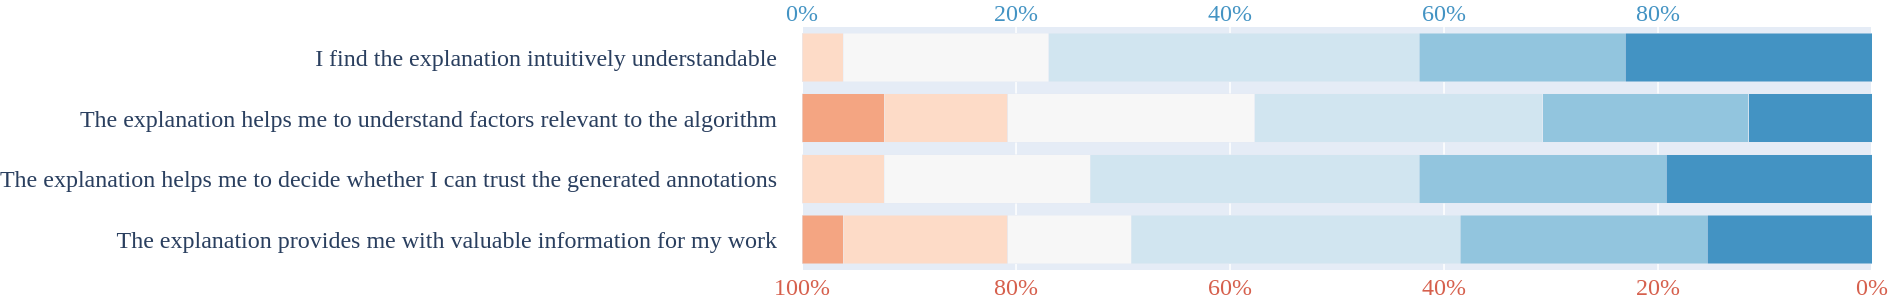
\includegraphics[width=\linewidth]{main/Graphics/4ResultsandAnalysis/0_TrustScores.png}
    
    Counterfactuals (One-axis):
    
    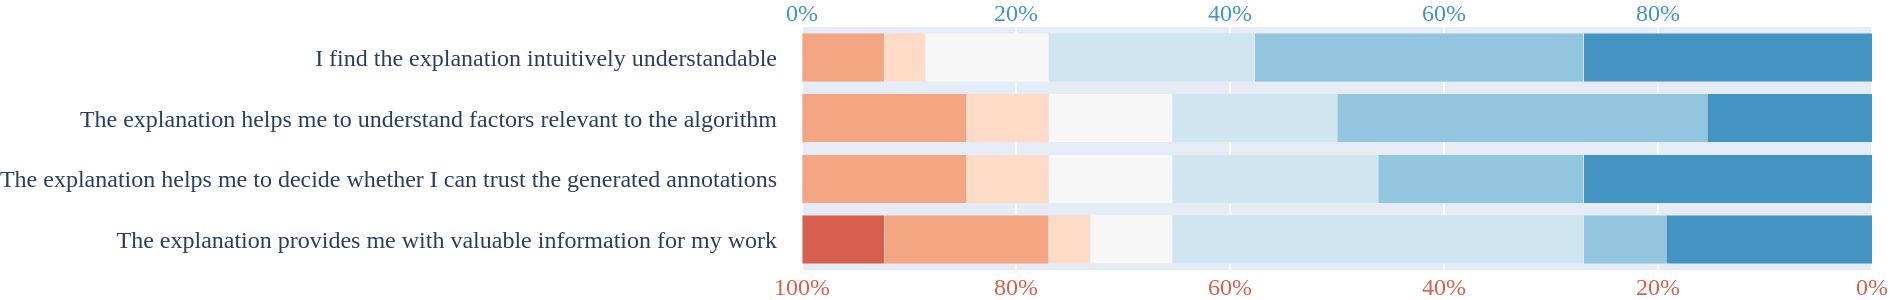
\includegraphics[width=\linewidth]{main/Graphics/4ResultsandAnalysis/1_CounterfactualsOneaxis.png}
    
    Concept Attribution:
    
    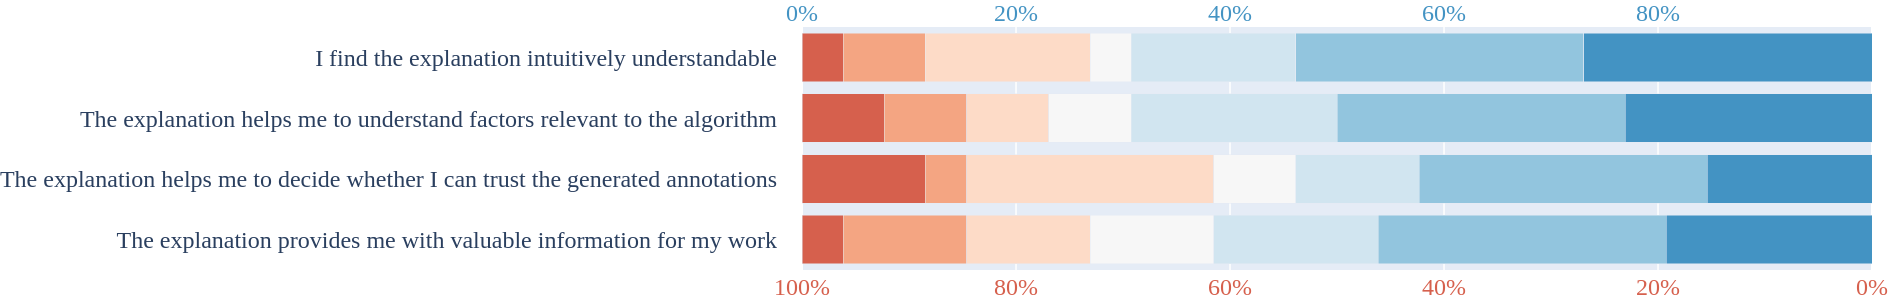
\includegraphics[width=\linewidth]{main/Graphics/4ResultsandAnalysis/2_ConceptAttribution.png}
    
    Counterfactuals (Two-axis):
    
    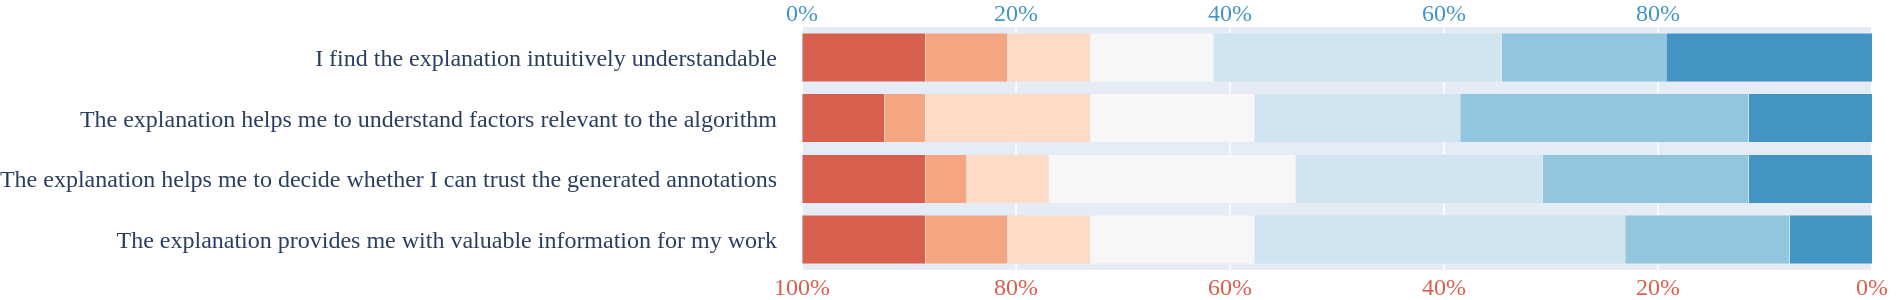
\includegraphics[width=\linewidth]{main/Graphics/4ResultsandAnalysis/3_CounterfactualsTwoaxis.png}
    
    Prototypes:
    
    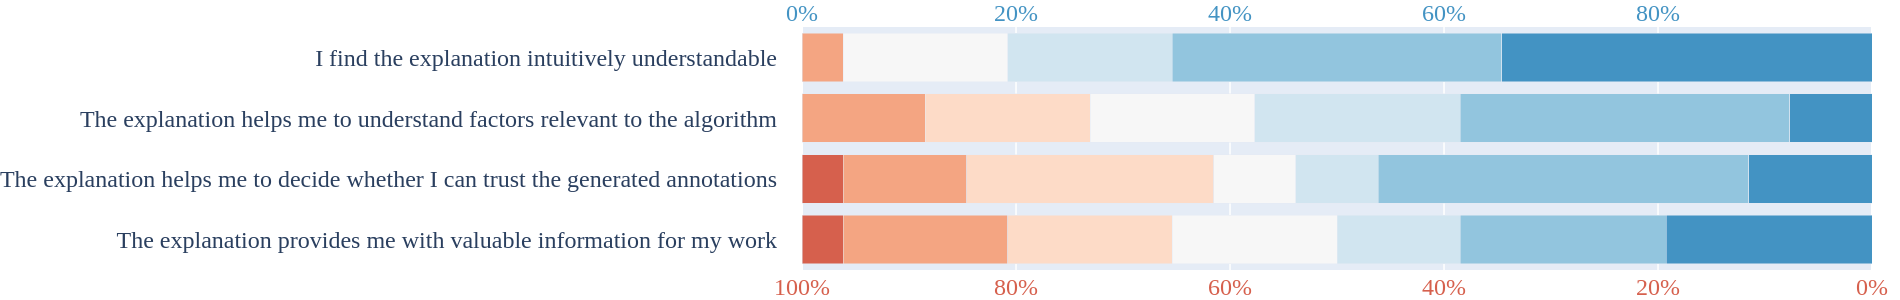
\includegraphics[width=\linewidth]{main/Graphics/4ResultsandAnalysis/4_Prototypes.png}
    
    Saliency map (Global):
    
    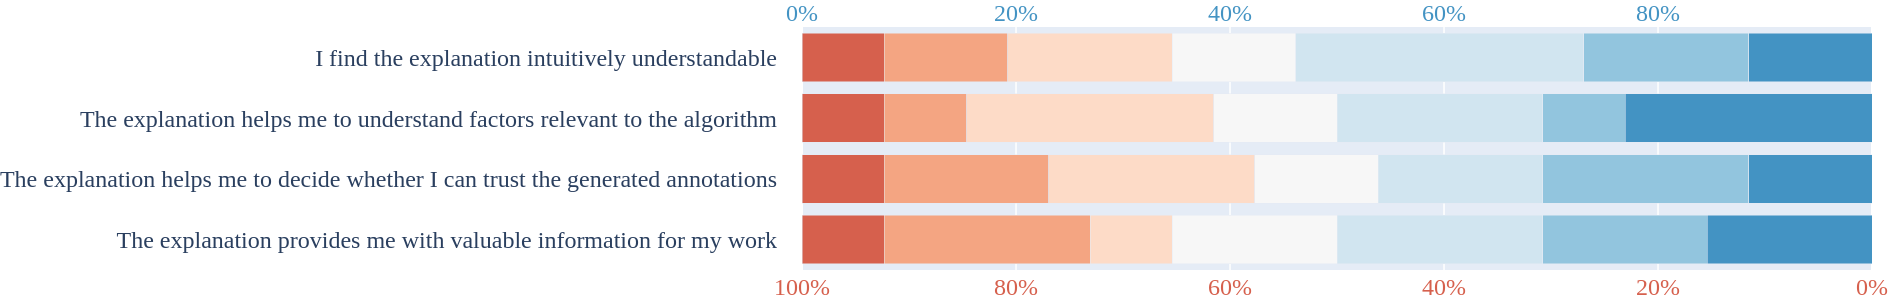
\includegraphics[width=\linewidth]{main/Graphics/4ResultsandAnalysis/5_SaliencyMapGlobal.png}
    
    Saliency map (Local):
    
    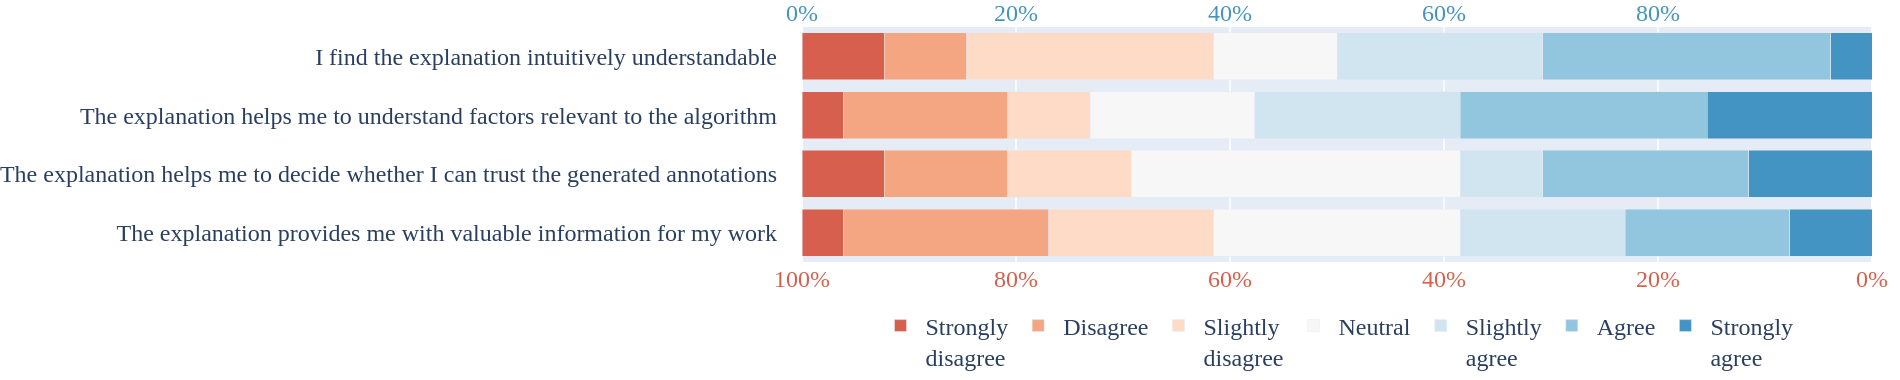
\includegraphics[width=\linewidth]{main/Graphics/4ResultsandAnalysis/6_SaliencyMapLocal.png}
    \caption{Distribution of responses from 25 admitted online questionnaire submissions.}
\label{fig:results}
\end{minipage}
\end{figure*}

The results of the online questionnaire are shown in Figure~\ref{fig:results}. Each bar shows the proportion of responses to the four Likert items shown relating to each of the explanation examples shown in Figure~\ref{fig:classes_overview}. Explanation examples are presented in descending order of positive responses (from \textit{Slightly agree} to \textit{strongly agree}) to the fourth Likert statement: ``The explanation provides me with valuable information for my work''. Trust scores were the most widely accepted explanation by this metric, while the explanation receiving the most positive median response was the one-axis presentation of counterfactuals.

\subsection{Interview participants}

Six board-certified pathologists (denoted P1--6) participated in video interviews, each lasting around 60 minutes. All interview participants were involved with research in pathology in some capacity, and three were currently involved in routine clinical practice. Years of experience as a certified consultant ranged from one to 45, with one participant being the current director of pathology, another a retired director, at major German research hospitals.

All participants of the interviews were familiar with the field of digital pathology and had some contact with AI applications, both in the research context (P1,\,2,\,5,\,6) and the applied and regulatory context (P3,\,5,\,6). Three participants reported being familiar with AI, but only having limited knowledge of the internal workings of it (P1,\,2,\,5). Furthermore, two participants (P5,\,6) reported having applied AI solutions to routine diagnostic tasks, albeit with unsatisfactory results. P3 and P4 had not seen or completed the questionnaire beforehand; all other participants had.

To preserve the anonymity of the participants, the video recordings and transcriptions are not made available in the public sphere. Anonymized excerpts from the original transcripts may be made available by special request to the corresponding author.

\subsection{Interview findings}

Approximately 360 minutes of interviews were recorded, transcribed and analysed. The resulting findings are presented here, grouped according to explanation class. Comments and observations not directly related to any of the explanation classes described were grouped according to topic and are presented at the end of this section.

\subsubsection{Saliency maps}

The reaction of interview participants to these two explanation examples ranged from explicitly stated as being difficult to understand, distracting or confusing (P1,\,2,\,5) to being trivial to understand but not at all useful (P6). Some participants found the explanation interesting but did not know exactly what to interpret from it (P4,\,5). One participant pointed out that it was unclear what was meant by 'the most relevant pixels' (P6).

Many participants identified factors important to the AI solution based on the pixels highlighted as most relevant, including presence, staining, size, and position of the nucleolus, or the staining pattern within the nucleus (P2,\,3,\,5,\,6). It was also pointed out that the explanation was ambiguous: it was not possible to infer which of these different factors were actually important or implied by the explanation (P2,\,5,\,6).

While it was indicated that the congruence between their understanding of what parts of the image are important with those highlighted by the saliency map would help them decide whether to trust the output (P3), most participants did not see this as a meaningful means of establishing the trustworthiness of the AI output (P1,\,2,\,4--6). It was pointed out to be confusing and/or distracting when saliency map and annotations did not align (P4) and redundant when they did; i.e., not understanding “what is output and what is explanation” (P1). 

The majority of participants did not find this type of explanation valuable to them at all for this task (P1,\,2,\,4--6). Even for those who thought it had some value in explaining the factors important to the AI solution, the modality was too detailed and/or too time-consuming (P4--6). Some thought that it might be useful in research (P4) or as just one component in an xAI toolkit (P3).

It was suggested that this form of explanation may be more suitable for classification tasks, where spatial features are more important than for the Ki-67 quantification case (P1,\,2,\,4,\,5). For instance, in the case where the output of an AI solution is the classification of a tumor over a large region. It was suggested that a pathologist could be more likely to trust a solution if the salient regions indicated match their expectations (P1,\,3).

The risk for positive confirmation bias with such explanations was also pointed out. ``[It] is hiding a lot of information. But it's very tempting, because it's very simple" (P1), particularly for pathologists not familiar with techniques with which they are generated or at least aware that there are many different ways to do so (P1). It was suggested that this type of explanation should only be used as one element within an array of explanations or as a final check (P1,\,3).

\subsubsection{Concept attribution}

This example was widely considered intuitively understandable and informative about the factors important for the AI output, albeit with limited value ascribed to this information (P1,\,2,\,4--6). Despite this ambivalent response, some pointed out that it would instill trust the AI output anyway (P2,\,6); i.e. that ``seeing the same factors that I find important makes me more confident in using the information that is provided, if I know that the application uses the same information that I would, as a human being. And applying the procedures that you are applying" (P6). 

% This sentiment was reinforced by the questionnaire results, where 68\% of respondents agreed that the explanation was intuitively understandable (statement 1), with a weak rank correlation between this and its perceived value to the user (\(\rho = 0.38\)). 

It was suggested that this explanation has some value as a sanity check, making clear whether a critical factor is being `missed' by the AI solution. However, in both cases, it was also pointed out that such sanity checks should hopefully be redundant once a pathologist was working with a well-validated, clinically approved solution (P1,\,4).

Criticisms of the explanation were the lack of precision and/or descriptiveness (P1--3) that having to read text is generally undesirable in the pathologist workflow (P3,\,4) -- i.e., that ``a picture is worth more than a thousand words" P3 -- or that it is simply unsuitable with the task of Ki-67 quantification (P2,\,4--6). 

It was pointed out that the explanation does not describe \textit{how} these factors affect the results, where the thresholds are, or how you would have to change them in order to get a different result (P1,\,6). A comparison was drawn between how a pathologist would explain what was important to them using descriptive language and that this falls short of that level of precision (P1).

Nonetheless, it was suggested that the explanation method is fundamentally promising and could be valuable with refinements (P2--6). Suggested improvements included showing factors in combinations (P2) and/or with finer granularity (P6), or moreover, with indications of thresholds and visual examples demonstrating how these changing factors affect output (P2,\,6), or in combination with an interactive tool for changing these thresholds (P6). 

It was suggested that this type of explanation may be more suitable for other diagnostic tasks; for example, in tasks involving differentiation between metastases and lymphocytes in lymph node sections, where other factors such as cell size and regularity are more important than in the Ki-67 quantification case (P2,\,4--6).

While narrative report generation through identification of text attributes was not deemed to be particularly useful (P1,\,5), the use of text-based explanations or descriptors to the generation of synoptic reports was mentioned (P3,\,5,\,6). 
% This is discussed further in section~\ref{sec:otherideas}.

\subsubsection{Prototypes}

The majority of participants found this explanation intuitively understandable~(P1,\,2,\,3,\,6). The explanation was described as “precise, short and understandable, and reflecting the thinking of pathologists” (P3); “Simply understandable for a human being” (P6).

% , with 80\% of the latter agreeing with the first statement to this effect. However, this ease of intelligibility correlated poorly with its perception as being a valuable explanation (\(\rho_{1,4} = 0.31\))

Aside from helping the user to understand the ``perfect positive and negative result" (P1); ``heaven and hell" (P6), many participants also drew conclusions from this explanation about the specific factors that were important to the AI solution. For instance, that the prototypes shown underlined the importance of staining intensity over other factors~(P2,\,6), ``size, shape, structure and color -- these are also the features you would focus on as a pathologist” (P3), or even indicated where the threshold between positive and negative annotations lay~(P5,\,6). One participant pointed out that the explanation did not explain why cells were detected as tumor cells (P4).

All participants expressed at some point that seeing prototypical examples can help to inform a user's trust in the AI output, with some explaining this with respect to whether they reinforced the idea that the solution was taking into account the same factors as a pathologist~(P1,\,3,\,4,\,6); “you feel better if you understand that the computer is evaluating something that you also do evaluate”~(P6); ``If the [prototype] is not fitting to my understanding [of what it should look like], I know that the result can't be right"~(P4). 

Despite this, there was little consensus that this type of explanation was valuable, with the common criticism that prototypical results do not reflect the diversity that is central to pathology~(P1,\,5,\,6) and/or that the information communicated is too trivial to be useful~(P5). Some participants who identified the explanation as having some value in informing trust in the AI solution later retracted this statement after identifying that the prototypes do not give an indication where the boundary between classifications lies, despite their expectations to the contrary~(P2,\,5); ``If you show me the prototypical positive result, I would expect anything less to be negative" (P5). The risk of positive confirmation bias was pointed out by several participants~(P1,\,2,\,5), leading one participant to name this as ``maybe the worst [explanation]" due to its potential to mislead~(P5).

One participant offered the alternative perspective that having the prototypical results was valuable as an indicator of glass slide quality, more than the quality of the AI output; i.e. if the prototypical examples do not match the pathologist's expectations, it can indicate that there is an issue with the slide preparation and staining (P4).

Several participants suggesting, either implicitly or explicitly, that a counterfactual-based explanation would be a more practical extension of this type of explanation~(P1--3,\,5,\,6), either citing the examples presented or describing their own variation on this theme. One participant suggested that it was helpful to have both types of explanation together, with the implied option of being able to switch between them (P3).

It was suggested that this type of explanation may be more suitable for tasks involving automatic detection of several similarly-presenting cell types, distinguishable only at high magnification (e.g. lymphocytes and plasma cells). In this case, having the prototypical examples of each cell type could give the user confidence that the AI solution  correctly resolved the different cell types without the need for laborious manual inspection (P1).

\subsubsection{Counterfactuals}

All interview participants indicated to some degree or another that the one-axis variant is immediately understandable; ``within a fraction of a second, I can see whether I agree with this or not" (P5); ``Immediately I know why half of the (negative) cells are missing" (P1); with many indicating that the two-axis explanation was not as clear as, or potentially more confusing than the simpler variant (P2--5). 

Interviewed pathologists were almost unanimous in their agreement that the explanation ``helps me understand what the algorithm is looking for” (P1), going so far as to claim that ``this is enough to understand [the result]" (P3). All participants drew some concrete conclusions about the factors important to the AI solution, finding it self-explanatory that staining was the most important factor distinguishing positive nuclei from those marked negative, with some identifying other important factors such as shape, size of nuclei, particularly in separating the positively annotated from the unclassified nuclei (in the two-axis example) (P1--3).

The ability to clearly see the boundary between positively and negatively annotated nuclei was widely considered as an important aid to trusting the AI output for the specific task of quantifying Ki-67 positivity of cancer cells. It was noted that there is another aspect to this task, in deciding which of the nuclei in the slide belong to tumor vs. non-tumor cells. 
Some indicated that the two-axis variant helped them to trust that the solution was making this distinction based on the right factors (P3), or at least, was having the same difficulties in making this distinction that they would (P1,\,5). One participant also suggested that this is not an issue, as the recognition of tumor vs. non-tumor cells is a separate upstream task that would have already been completed by this point ``Once I'm at IHC, I'm just looking at positive or negative''~(P5).

There was a consensus amongst participants that these explanations, or at least the one-axis variant, were a valuable method for understanding and knowing whether to trust the AI output for this particular task. Referring to the two-axis variant, one participant stated, “I think ... this one is the one that provides me all the information I need to assess the results that the algorithm is giving me, based on my own way of accessing [this task], and the pitfalls that I know are there ... because it's also all the information that I use on my own" (P1); another ``I know [artefacts] aren’t being included in the decision because they aren’t shown in the explanation"~(P3). 

Many participants noted that the one-axis case could be more useful due to its simplicity (P2--5), a sentiment backed up by the questionnaire results, in which the two-axis variant rated significantly lower on Q1.

Aside from this, other pitfalls were noted by participants. It was not self-explanatory that the intermediate images were synthetic (P2) and it was not clear which other factors apart from staining intensity were changing between the positive and negative cases in either variant~(P2,\,3). It was also suggested that the explanation could be distracting, causing a pathologist to spend too long scrutinising the exact position of the decision boundary shown in the explanation, at the expense of looking at the slide itself~(P4).

It was suggested that the explanation could be improved by showing an ensemble of counterfactuals to try and explore the different factors that are changing between positive and negative~(P2,\,6). It was also suggested that the on-slide control should also be displayed for comparison~(P6).

Many participants mentioned the possibility of interactivity, with one taking it a step further, suggesting that this explanation should only be used as a tool to  refine the decision boundaries interactively, not as a source of explanation in itself~(P6). Along these lines, they also suggested that this would be a valuable tool for refining multi-modal decision boundaries, e.g. in HER2 grading where, unlike Ki-67, the intensity of staining identified as positive has clinical implications.

\subsubsection{Trust scores}

The labelling of annotations as high- or low-confidence was regarded as being intuitively understandable. Aside from identifying the AI solution's confidence in its annotations, many participants also inferred from this the factors that may have been important to the solution, linking low-confidence annotations to the presence or absence of certain features (P1--3,\,6); e.g. ``[I] can see from this that the staining intensity was important, but the size was not'' (P6).

% , a sentiment corroborated by 76\% of the survey respondents (see Figure~\ref{fig:results}), even as being described as ``almost too basic [to be considered an explanation]'' (P5). % TODO: decide whether this is how we want to use the questionnaire results.

All interview participants indicated that seeing the confidence of annotations (or at least, those that were low confidence) helped them decide whether to trust the results. On the one hand, this stemmed from the implied ability to choose what to do with these low-confidence annotations, e.g. to accept, discard or manually change them (P1--5) or to further refine parameters and thresholds (P6). On the other hand, the coincidence between annotations that were labelled low-confidence and those that the pathologist would also ``have difficulties with" (P1) also increased trust in the AI solution (P1,\,2,\,5,\,6). One participant explained this in terms of giving them the feeling that the AI solution was ``doing the same things that I do" (P2). 

Overall, being able to see the low-confidence annotations was deemed valuable by all participants to assess the AI output, particularly in conjunction with other explanation methods (P4--6), or as a final check before deciding whether to accept the results (P6). Some expressed this in stronger terms ``the way it is presented, I would know at a glance whether I accept this evaluation" (P6); ``[I can] take a glance and say ‘this fits with my interpretation’" (P5). As well as the expectation of the ability to manually resolve low confidence annotations, it was also presumed that this feedback would (or should) train and improve the AI solution (P1,\,6).

In terms of criticism for the approach, it was suggested (P2,\,3) that an effective implementation would require confidence indicators for all classes of annotations. A proposed improvement to the implementation shown would be to display low/high confidence annotations for both positive and negative annotations (P2,\,3); for instance, separately or using different color schemes. 

Aside from confidence scores on a per-annotation basis, information about overall model confidence, including details of validation performance, training data, etc. was identified as an important factor for building trust.

\subsubsection{Use of AI in pathology}

It was observed that the term `AI' is vague,  particularly in light of the EU's developing regulatory terminology~\cite{ISO_IEC_22989}; ``Nobody knows what is artificial intelligence. Nobody knows what ... intelligence [is]" (P3). It was noted that, according to such definitions, AI has been applied to pathology for decades in the form of numerical modelling, regression, etc. Similarly, computer-assisted diagnosis has existed in some form or another for many decades, with image processing methods, counters, microscope-mounted cameras, etc., and the modern trend of deep learning applications to digitized slides was regarded as the logical next step in an ongoing process of innovation (P1,\,3).

AI solutions were often regarded as an extension of technology applied by pathologists for decades, numerical modelling, counters, microscope-mounted cameras, etc., assisting with simple but time-consuming tasks (P1,\,3,\,6); e.g. counting cells or estimating percentages. Speed was often named the highest priority for AI solutions, with the rationale that if the AI did not save the pathologist time, they would simply perform the task themselves (P4--6). The slide digitisation process itself was also named as a limiting factor; i.e., by the time a slide had been scanned and was ready to be viewed digitally and/or processed by an AI solution, the pathologist could have already completed the task under a microscope (P4). It was suggested that slide digitisation needs to reach a critical level of adoption ``over 90\%'' in order for such applications to make sense (P6).

Two participants expressed the opinion that the pathologist's liability for their decisions, and therefore the obligation to check every result and slide anyway, was limiting the usefulness of AI solutions (P4,\,6). It was suggested that AI solutions could be helpful as a backup, giving a second opinion or flagging features worth reviewing, even after the pathologist has made their own diagnosis. To this effect, the impartiality of AI solutions (for instance, to the seniority of the pathologist) was cited as a strength (P4).

Regarding the state of AI in pathology, limitations regarding accuracy (P5) and data protection (P6) were cited as prohibitive for the use of commercial solutions in clinical settings. It was observed that ``you cannot [just] buy it at the App Store" (P3), rather than machine learning techniques must become part of pathologist's training in order for AI to be effectively applied to pathology, and that the lack of mutual understanding between computer scientists and pathologists was a major factor limiting adoption (P3,\,5).

% Mesothelioma detection solution, good prognosis prediction, but not clear what features are being used. “Not sure who is learning here, we or machine” P5

The issue of inter-pathologist variability in Ki-67 positivity quantification was identified; ``[It] is very boring to count positive or negative nuclei. And most of these things are now based on estimations only, and therefore the results are very weak .... in breast pathology, there's a threshold of Ki-67 positivity of 14.4\%, for selecting some kinds of patients to get chemotherapy or not, and nobody can [estimate] 14.4\% ... but it is the official recommendation of some bodies in European and national pathology, breast oncology" (P1).

Some participants considered AI assistance to be a useful tool in mitigating this issue (P1--3), citing the ability of AI solutions to work systematically without becoming fatigued (P1,\,3) and the potential for them to make better estimations by taking into account other data modalities; e.g. cell morphology, or molecular data (P2). 

Conversely, it was suggested that this task was too trivial for AI assistance to be practical (P6) or that lack of standardized training data represents a prohibitive limitation to their potential accuracy (P3). Another participant identified that the pathologist's fine-tuning of AI parameters (e.g. positivity threshold) would anyway reintroduce the same subjective variability, should they have this option (P2).

\subsubsection{Trust in AI}
\label{sec:trustinAI}
The pathologist's own judgement was cited as the primary basis for judging the accuracy, and therefore trustworthiness, of an AI system (P5,\,6). It was suggested that pathologists' trust in an AI solution would be established after extensive use, testing, and comparison with the work of multiple colleagues (P5).

External validation was commonly identified as a critical prerequisite to trust in an AI solution (P1,\,2,\,4,\,5). It was suggested that AI solutions can and should be subject to more forms of validation than the work of pathologists normally would (P2). Diversity (P1,\,5) and experience (P6) of annotating pathologists were stressed as critical factors in assessing the quality of validation and/or training data. Annotations from three pathologists, preferably all from different institutes, was suggested as a minimum requirement for trustworthy ground truth data (P1,\,5).

Participants expressed a range of attitudes toward relinquishing control of the decision-making process to an AI solution. Most participants expressed openness to an AI solution giving a contradicting result to their own (P1--5), with some identifying benefits in giving an AI solution more control over the decision-making process (P1--4), provided it was shown to be reliable. In contrast, one participant expressed the expectation of always having control over the decision boundary of an AI solution, although suggested that the parameters set by an experienced pathologist might then be used with confidence by one with less experience (P6).

The pathologist's legal accountability for their decisions was explicitly mentioned several times (P4,\,6) and used as a rationale both for (P4) and against (P6) endowing more control to an AI solution. 

\subsubsection{Expectations of explanations}

Participants unanimously expressed a preference for simple, visual explanations; "Pathologists are always looking for visual things, matches thinking. Anything outside this modality is foreign" (P1).  Interactivity was often cited as a desirable (P1,\,3,\,4), with one participant suggesting that all of the explanations shown should only be presented as tools with which to interact and manipulate the AI solution, never as a ``source of truth'' (P6).

All participants at some point expressed that explanations tended to increase trust in the AI solution when they demonstrated it making decisions in a relatable manner; i.e., when ``it matches the way we  think when we see the image" (P1). There was a common tendency for participants to attribute relatable decision-making processes when presented with explanations of the AI result; ``We are testing it like we would another pathologist" (P1).

It was mentioned that it is often challenging for pathologists themselves to explain the factors that were important to their own diagnostic decisions, that there is a certain amount of experience and intuition involved (P1,\,2), and that a lack of standardized descriptive vocabulary is also a limitation (P3). However, it was also pointed out that ``we all have passed some information to other pathologists, otherwise there would not be pathologists today" (P1). The method described by one participant for explaining their own decisions would be multi-modal: a region of interest, simply annotated, coupled with high-magnification insets to highlight key features (P6).

% Over the course of the interviews, participants suggested several potential approaches to explain or augment AI solutions for pathology. 

Several participants described variations on the theme of structured annotations (in the style of synoptic reporting) for the slides in question, providing additional context with which to evaluate and confirm the AI output (P2,\,5,\,6). For instance, allow a pathologist to quickly compare descriptors for regions marked by an AI solution as healthy vs. unhealthy (P6). It was implied that these annotations could be automatically generated, either based upon a body of machine-readable ground truth data (P6) or by combining the results of many other feature detection algorithms (P2). 

Automated anomaly detection was also mentioned, wherein an AI solution might -- either as or supplementary to, some other diagnostic output -- flag up features that are statistically rare and/or out of distribution for their training data for manual review (P4,\,5).

An approach was suggested, wherein an AI solution could `explain' its decision by showing the images from training data that were most important for a given outcome, comparing this process to that of a pathologist referring to previous cases and reference material to justify their decisions (P1).

Aside from, or in addition to, any explanation of AI outputs, it was suggested that a ``brochure" containing important information about a given solution would be desirable for building trust it in. Suggested content included: the size of the training dataset, sources of annotations (see section~\ref{sec:trustinAI}) and molecular data, and accessible explanations of the methods employed (e.g. machine learning architectures) (P5). 